\setAuthor{Aigar Vaigu}
\setRound{lõppvoor}
\setYear{2023}
\setNumber{G 3}
\setDifficulty{3}
\setTopic{TODO}

\prob{Lääts ja kaks peeglit}
Konstrueerige objekti $AB$ (vt joonist lisalehel) kõik kujutised. Skeemil on hall sein, sinine \SI{45}{\degree} kaldu poolläbilaskev peegel (pool valgusest läheb otse läbi, pool peegeldub nagu tavalises tasapeeglis), kumerlääts fookuskaugusega $f$ ja tasapeegel. Lahendage ülesanne lisalehel.


\hint

\solu
\par
Tõmbame punktist $A$ väljuva horisontaalse sinise kiire, pärast poolläbilaskvas peeglis peegeldumist on see vertikaalne, läätses koondab selle optilisele peateljele, kus see peegeldub ning jõuab läätseni tagasi. Teiseks kiireks tõmbame lilla kiire punktist $A$ poolläbilaskva peegli keskpunkti, pärast läätse läbimist liigub see edasi otse (kuna läätse fookus on poolläbilaskva peegli keskpunktis) ning lõikub läätse tasandis algse kiirega. Selle punkti näol on tegu $A$ kujutisega. Analoogselt konstrueerime punkti $B$ kujutise läätse tasandis. Objekti $AB$ kujutis läätse tasandis on sama suur kui oli algne kujutis. Tasub märkida, et seda kujutist näeb ülevalt vaadates (kui oleks tegu tavalise peegliga näeks seda ainult poolläbilaskva peegli ja läätse vahel asudes).

Nii algsel objektil kui selle kujutisel läätse tasandis on ka kujutised poolläbilaskvas peeglis nagu oleks neil tavalistes peeglites. Konstrueerime ka need.

Kokku tekib kolm kujutist. Ülemist kujutist näeb altpoolt poolläbilaskvat peeglit vaadates. Parempoolset kujutist näeb vasakult poolt poolläbilaskvat peeglit vaadates. Nagu juba mainitud, siis kujutist läätse tasandis näeme vaadates ülevaltpoolt.

Kuna siin skeemis on poolläbilaskev peegel, siis kujutised on mõnevõrra tumedamad võrreldes tavalise peegliga. Alumine kujutis 2 korda tumedam vaadates seda poolläbilaskva peegli ja läätse vahelt ning 4 korda tumedam vaadates seda läbi poolläbilaskva peegli. Parempoolne ja ülemine kujutis on mõlemad 4 korda tumedamad.
\begin{center}
  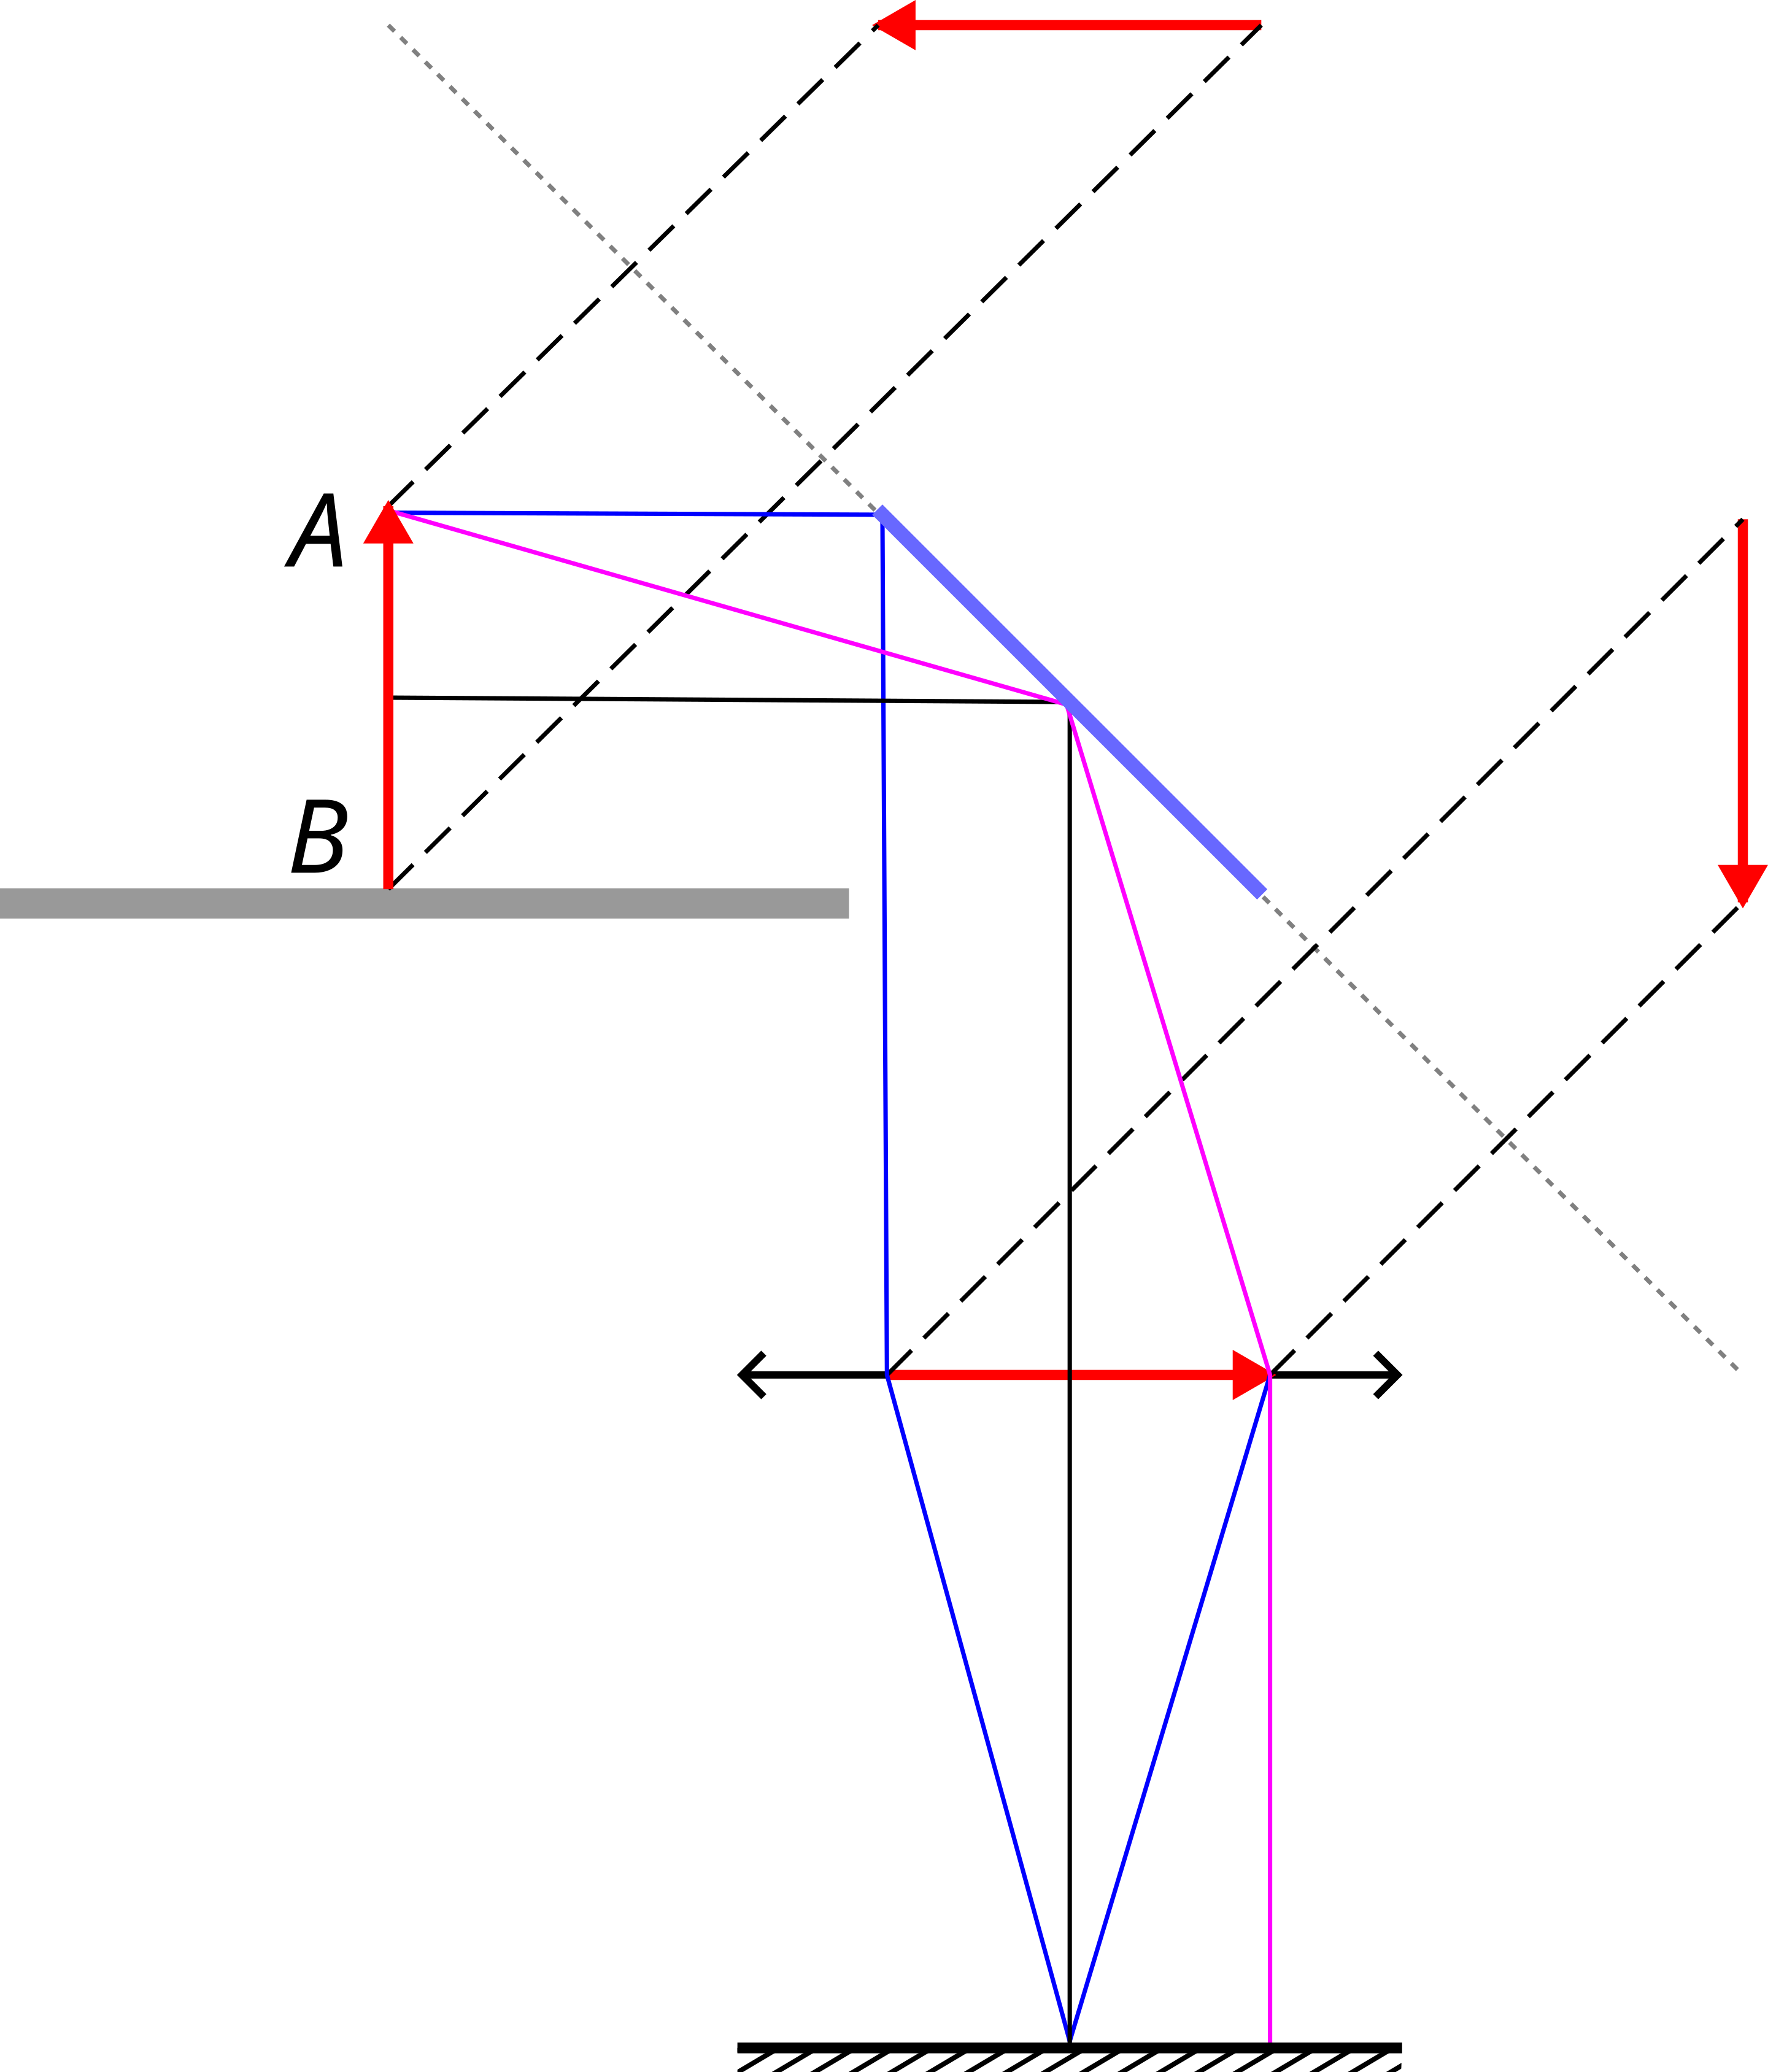
\includegraphics[width=0.86\textwidth]{2023-v3g-03-sol.png}
\end{center}
\probend